\chapter{重修线性代数10——计算}

线性代数源于解线性方程组,这是数学公式逆向的计算。在计算机时代之前,限于手工计算的能力,线性代数多是作为理论研究的基础。到了现代,它已是理工科但凡涉及到统计和数值计算必备的工具了,最近更成为机器学习热门的基础课。

\section{病态系统}

数学的理论无论多么漂亮,应用到实践,总要落实到数值的计算。线性系统是最简单实用的数学模型,理论上解线性方程组有非常确定的结果,但也可能有意外。让我们看一个例子。

\kaishu

解线性方程组0.410x + 0.492y = 0.902,0.492x + 0.590y =1.082;得x=1,y=1. 若第一个方程右边的0.902略有变动成为0.901,解就变成x= 4.5976,y= -2.000; 同样第二个方程右边的1.082的数值变成1.081后,解就变成x= -2.000,y= 3.500.

\songti

实践中的数据总有些误差,方程的参数微小的变动,竟让计算结果面目全非,这确实让人始料不及。这样不稳定的计算结果在应用上毫无价值。问题在于,这个差异并非是计算误差造成的,将它们代入方程验证都精确无误. 这就无从计算上来改善了。这种对参数微小变动敏感的系统称为是病态的(ill-conditioned),这是数学模型的问题。这个例子,在几何图像上不难看到原因。每个方程在空间确定一条直线,方程的解是这两条直线的交点。这两个方程确定的直线近于平行,所以位置略有变化(红线和绿线),它们的交点(红点和绿点)的位置就差得很远。

% TODO: \usepackage{graphicx} required
\begin{figure}[h]
	\centering
	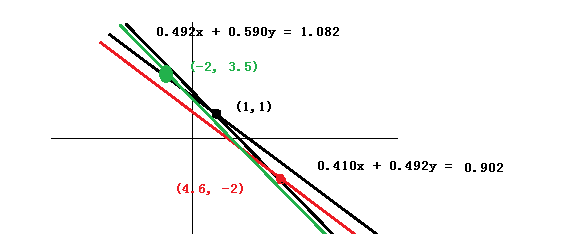
\includegraphics[width=0.7\linewidth]{pic/1612386nrnueyrye6k8kq4.png}
	\caption{一个病态系统的例子}
	\label{fig:1612386nrnueyrye6k8kq4}
\end{figure}

在数值分析中,条件数(conditionnumber)用来描述数学模型系统的微扰对计算结果的影响。大致说来,对条件数κ,$ log_{10}κ $是你在计算可能要丢掉的数字位数$ (log_{10}\|Δx/x\|\leq log_{10}κ+ log_{10}\|\delta b/b\|) $,当然这个数κ是很难确定的,它是作为相对误差上界的估算。对于解线性方程组 Ax=b,它的意思是$ \|\delta x/x\| \leq κ\|\delta b/b\| $,经过推导有$ κ(A) =\|A\|*\|A^{-1}\| $,对通常的$ L_{2} $范数$ κ(A)= |\sigma_{max} /\sigma_{min}| $,它是A做奇异值分解后最大与最小奇异值之比,在可对角化的矩阵即是最大绝对值的特征值与最小绝对值的特征值之比。正交阵(或酉阵)的条件数是1,这是最小的矩阵条件数值,所以正交阵具有最好的计算稳定性。这说明我们建立线性的数学模型时,要尽量选择近于正交的数据来建立方程组。

在MATLAB或Octave可以用cond(A)指令计算A的条件数。上面例子中κ(A) = 6099.6.

\section{支点对计算的影响}

高斯消去法几乎是线性代数各种计算的基本手段。它不仅用来化简矩阵计算行列式。对线性方程组的求解,把方程右边的列向量拼入左边的矩阵,成为增广矩阵(A,\textbf{b}),然后对它进行行间的变换,直至左上角部分变成三角阵,然后对照右边最后一列,判断方程是否无解,若有解则用右边三角阵部分迭代求解,多解时则同样可以迭代解出零空间的线性无关向量。

矩阵求逆,则把单位阵拼入左边成为增广矩阵(A,I),右边部分记录了所有的行变换,与解方程一样,先从上到下,用支点(pivot)即主对角线上的元素,消去对角线下非零元素,把左边部分变成上三角阵。然后从下到上消去对角线上非零元素。如果A是满秩的,增广阵终将成为$ (I, A^{-1}) $,右边即是逆矩阵。在这从上到下,三角阵化的消去过程中,只要支点是非零的,我们不需要交换行来进行,这时增广矩阵的右边的子矩阵是个下三角矩阵U,而左边是个上三角的子矩阵L,这时的增广矩阵(U,L)实现了LU分解。

理论上,只要这个过程中的支点是非零元,用消去法解方程、求逆和做LU分解都是可以的。实际上仍然会遇到问题。看下面用第一行消去第二行第一列,做的LU分解。

\[A=\begin{bmatrix} 0.0001&1\\ 1&1 \end{bmatrix}=\begin{bmatrix} 1&0\\ 10,000&1 \end{bmatrix}\begin{bmatrix} 0.0001&1\\ 0&-9999 \end{bmatrix}=LU\]

条件数κ(A)=2.6184尚属于良态,而$ κ(L) =10^{8},κ(U) =0.9999*10^{8} $,都是非常病态了,用这个分解做计算会带来很大的误差。问题在于计算过程中支点的数值太小,解决的办法是运用支点做消去法前,先搜寻支点所在位置及下面,从中选出最大元,交换这两行使得最大元在支点位置。对这个矩阵A,是先交换上下两行,然后再做消去法,这样有:

\[P=\begin{bmatrix} 0&1\\1&0\end{bmatrix},\;PA=\begin{bmatrix} 1&1\\0.0001&1 \end{bmatrix}=\begin{bmatrix}1&0\\0.0001&1\end{bmatrix}\begin{bmatrix} 1&1\\ 0&0.9999 \end{bmatrix}=LU\]

这时κ(L) =1.0001,κ(U) =2.6182,都是良态的。所以在矩阵的计算中,为了减少误差经常需要交换行或列,这个步骤可能隐含在算法中,也可能需要表示在计算机函数的式子里。通常用置换矩阵P来表示这些行或列的交换,如在MATLAB或Octave中指令 [L U P]=lu(A),指的是 PA = LU的分解。为了减少误差,分解指令[G U]=lu(A),如果需要交换行,则把P吸收在G中,$ G=P^{T}L,A=GU $,这时G不再能保持L的下三角阵的形式了。

\section{机器学习}

人们走向理性,依赖于在意识层次上的逻辑求证。不明因果机理的预测和难以追踪判断过程的结论,都被视为迷信而被科学排斥。算术曾经是解决实际问题计算唯一可靠的途径,在那里应用问题分门别类地归纳成不同的类型,诸如鸡兔同笼、宝塔装灯等等,每个计算步骤和所得的数量,都有直观可以理解的含义。代数的方法偏离了直观推理的途径走向抽象,三个未知数的线性代数方程,已经难以用单向逻辑推理的路径来追踪它解法的含义。我们只能用严格的逻辑,来证明每一步的代数运算都是等价或蕴含原来问题的不同描述。由此,我们可以用简化了问题的计算答案来回答原来的问题。在理性求证的过程中,我们把解方程的代数方法看成可以信赖的中间站,将现实问题的各种关系表示成方程后,放弃了对解法计算的每一步的追踪判断,直接承认它的结果。物理等科学研究沿用这种思想,把实际问题描述成数学模型后,直接依赖于数学的分析和计算。

机器学习将代数方法的启示推向另一个高度。它不再依赖于人力把实践中的预测和判断问题描述成一个数学模型,而是运用一个带有众多可调参数的通用数学模型,直接利用拥有的数据来调节参数自行寻找适用于这一类数据的具体模型,以此应用解答预测和判断问题。

与代数的方法取代算术方法的困惑一样,机器学习的调整模型参数及应用模型的计算机制,在数学上都是精确有效的。但巨大数量的可变参数,难以把这简单数学模型的一个具体的辨识判断过程,解析成为像物理规律那样单纯过程的因果性机制,无法用简单逻辑推演的跟踪来获得理解。机器学习的智能渐渐走离我们理性的监督,却成为未来应用计算的利器。下面简单对此作介绍。

机器学习与人类经验公式和分类的基本计算是一样的,都是用线性的方法计算参数,找出与实验数据匹配最小误差的数学模型,以此用来预测未知。对经验公式,用的是线性回归,找出那个线性函数,它是个与实验数据误差最小的的超平面;对模式识别的分类,用逻辑回归,找出那个判别函数,它是个分隔两类样本的超平面,与实验数据的误差最小。最后它们都归结为确定那个超平面的线性代数计算。(注:这里的超平面,指n维几何空间中的n-1维平面,它不是指那种过原点作为n-1维线性子空间的超平面。)

在n维线性空间中,满足内积$\langle \mathbf{z},\mathbf{a}\rangle = b $的向量\textbf{z},构成n维几何空间中的一个n-1维平面,将向量扩充到n+1维空间,令$ \mathbf{x}=(1,\mathbf{z}^T)^T, w=(-b,\mathbf{a}^T)^T $,这个内积可以表示为$ \langle \mathbf{x},\mathbf{w}\rangle= 0 $.

\begin{figure}[t]
	\centering
	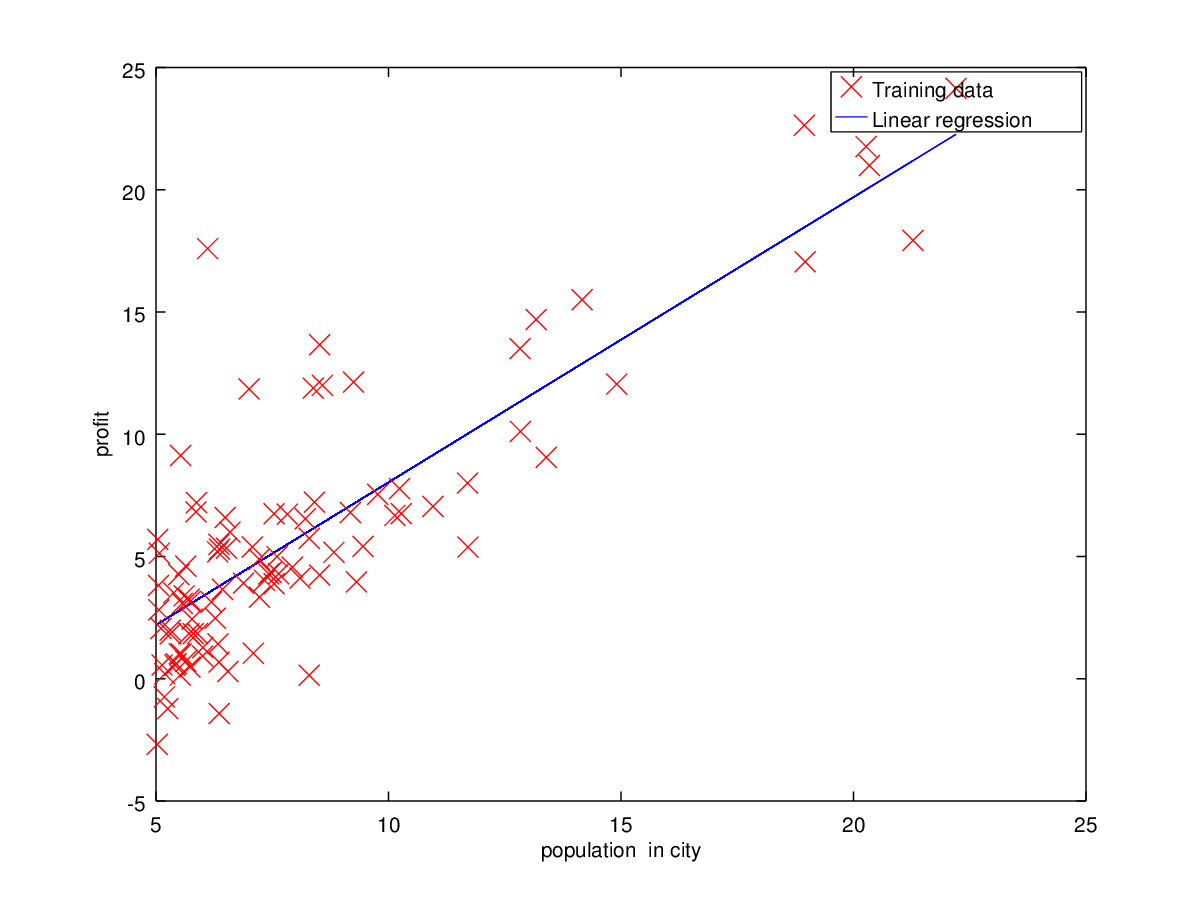
\includegraphics[width=0.49\linewidth]{pic/161238petg2epyqhslbulz.png}
	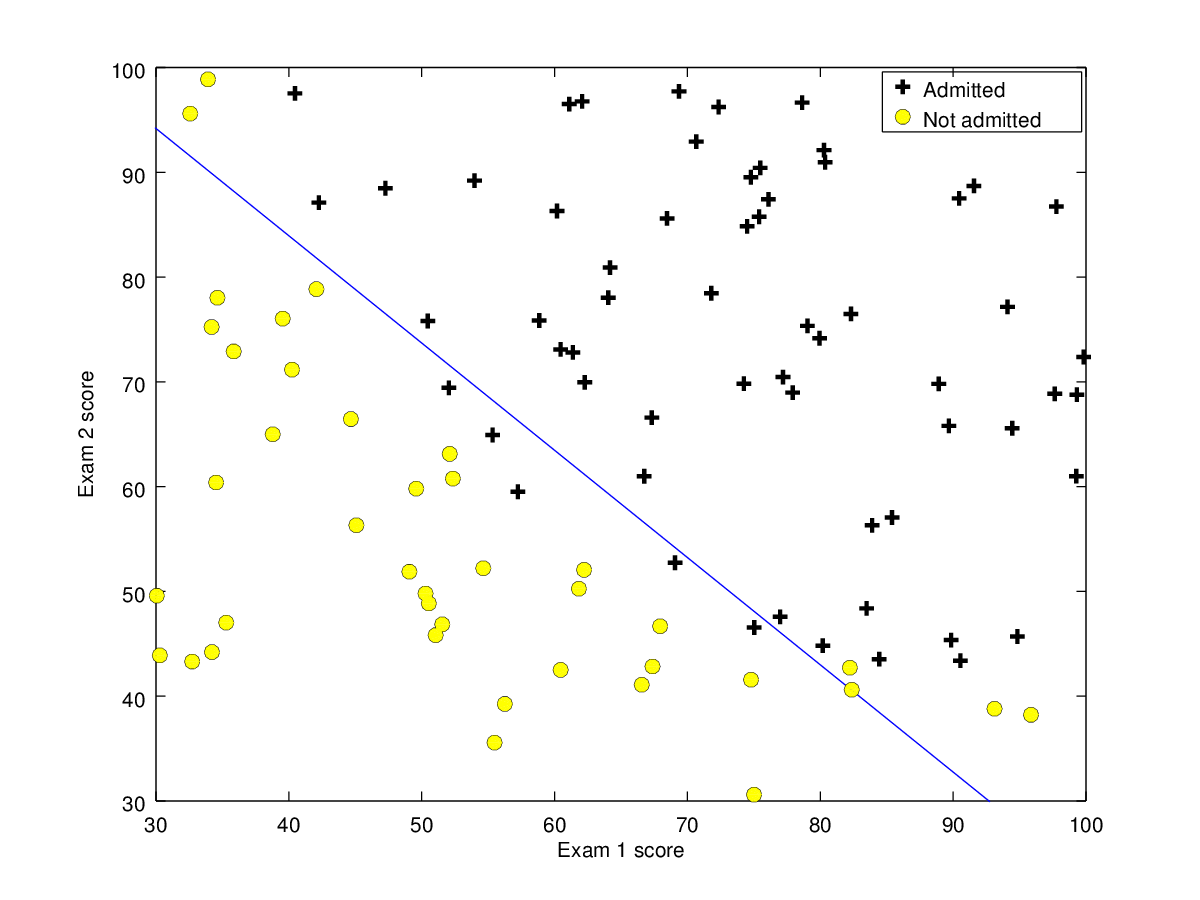
\includegraphics[width=0.49\linewidth]{pic/161239i3870x2cvwmclc09.png}
	\caption{线性回归}
	\label{fig:161238petg2epyqhslbulz}
\end{figure}

\textbf{线性回归(linear regression)}:在线性回归的数学模型中,假定有足够多描述事物的属性,表示为函数的变量,归纳了经验的数值公式是这些属性变量的线性函数,我们尽可能应用大量的实验数据,来统计出误差最小的模型的系数。具体计算如下。

假设n维的属性向量$ \mathbf{x}_{i} $和公式结果标量$ y_{i} $,经验公式有线性的关系$ \langle \mathbf{x}_i, \mathbf{w}\rangle = y_{i}$,其中w是待定的参数向量。我们有m组实验数据,m >> n,希望对所有的实验数据 $langle \mathbf{x}_i, \mathbf{w}\rangle$ 都非常靠近 $  y_i $ . 在上一篇中提到,这是列满秩矩阵解线性方程组的问题,可以用最小二乘法求解。

把m个n维行向量$ \mathbf{x}_i^T $写成m*n矩阵X,m个$ y_i $列成向量y。设误差函数$ J(\mathbf{w}) =1/2\|X\mathbf{w} - \mathbf{y}\|^2 = (X\mathbf{w} - \mathbf{y})^T (X\mathbf{w} - \mathbf{y})/2 $,计算问题是,求让$ J(\mathbf{w}) = (X\mathbf{w} - \mathbf{y})^T (X\mathbf{w} - \mathbf{y})/2 $取最小值的向量$ \mathbf{w_0} $.  

$ J(\mathbf{w})  $是个在n维空间中的二阶幂函数的曲面,它有唯一的极小值在梯度为零处,即梯度$ X^T ((X\mathbf{w} - \mathbf{y}) = 0 $,这可以表示成正规方程$ X^TX\mathbf{w} =X^T\mathbf{y} $. 它有唯一解$ \mathbf{w_0} =(X^TX)^{-1}X^T\mathbf{y} $.  在大数据的情况下,这个公式解的计算量太大,我们可以采用迭代的方式求解,这通常从任何一个w的初值开始,沿着这个梯度$ X^T ( X\mathbf{w} – \mathbf{y}) $下降的方向,迭代逼近这个极值点$ \mathbf{w_0} $.

\textbf{逻辑回归(logistic regression)}:模式识别是进行逻辑分类,它假定在足够多属性为坐标的多维空间中,用一个超平面把空间分成两半,分别对应着不同的逻辑值。逻辑回归用来确定这个将实验样本中分类误差最小的超平面。

在n维线性空间中,满足内积 $ \langle \mathbf{z}, \mathbf{a}\rangle = b $的向量\textbf{x},在\textbf{a}方向上投影的长度都是$ b/\|a\| $,这些x向量的端点构成的n-1维的平面,这超平面与原点的距离是$ b/\|a\| $。空间上面的点依指向它的向量\textbf{z}在\textbf{a}上面的投影被这超平面分成两个部分,依内积$ \langle \mathbf{z}, \mathbf{a}\rangle  $是否大于b,确定它们属于哪一类。这是模式辨识和机器学习中分类最为基本的直观图像。

采用上面扩充向量的符号,这个超平面是由\textbf{w}的数值来确定的,所谓的学习是用样本的数据$ \mathbf{x}_i $和对应的0或1的分类值$ y_i $,来计算这个\textbf{w}。数学模型的预测值是由判断函数$ g(\langle x,w \rangle ) $来确定,理论上$ g(\langle x,w \rangle )= (sign(\langle x,w \rangle)+1)/2 $,但为了便于计算梯度,多数取sigmoid 函数g(t)=1/(1+exp(-t)).

我们同样用求误差函数$ J(\mathbf{w}) =1/2\|g(X\mathbf{w}) - \mathbf{y}\|^2 = (g( X\mathbf{w}) –\mathbf{y})T (g( X\mathbf{w}) –$   $\mathbf{y})/2 $ 最小的方法,来得到极值点$ \mathbf{w_0} $,用迭代的方法沿着梯度下降的方向,逼近这个极值点$ \mathbf{w_0} $.

\section{世界是线性的吗?}

上一节说,机器学习的核心算法线性回归和逻辑回归,应用的都是线性模型。这也是经验公式和模式识别的基础。我们的世界都是线性的吗?

开篇时也说,令人感到幸运和疑惑的是,科学研究上凡是用到数学,有着漂亮定性和定量结果的,基本上可以变成一类线性系统,或者用它来逼近。为什么?

世界是线性的吗?其实不是,只是非线性的系统正向计算不难,但难以反向求解,更无法分部综合。我们能用数学工具取得很好结果的,基本上是线性系统。力学是线性动态系统,绝大多数电路是线性系统;描述连续介质,能量和场的波动,传导,稳定状态的数理方程是线性系统。非线性系统可以用两种方法将它应用线性系统的方法来处理。一是可以在足够小误差的邻域看成是线性的;微分几何用曲面上点的邻域,投影到与之相切的线性空间来计算;非线性动态系统控制稳定或跟踪已知轨迹时,可以用线性系统来近似。二是在应用上尽可能把系统处理成线性的,而把非线性部分局限在一小处或作为输入,以便分析和综合。难以照此办理的许多非线性系统即使有精确简单的方程描述,如混沌系统、联结主义模型,无论在定量和定性上,都难以深入。科学和技术与一切在竞争博弈中的发展一样,都是路径依赖的。某一方向取得突破,人们蜂拥而至,用先创的概念作为后建的基石,建构我们理解的世界。科学发展至今,解释事物的理论无所不在,我们似乎已经充分了解了这个世界,其实这不过是看见在科学这条高速公路旁的城镇,公路不可达之处是不可知的荒野。但是无论如何,线性代数已是现代科学知识的基础构件,我们必须能在头脑中想象它。

机器学习的线性模型怎么用在这个并非是线性的世界?线性回归怎么拟合一条曲线上的数据?怎么用一个超平面分划由一个曲面界定的类别?答案在于增加维数。空间中任意的样本点集,都可以看作是高维空间中点集的投影,它们可以在高维空间的一个超平面上,或被一个超平面分类。

例如,实验数据(1,4), (2, 9), (3, 20), (4, 37), (5, 60) 是二维空间的曲线 $ y = 3x^2 – 4x + 5 $上的点,在实验中增加一个属性$ x_2 = x_1^2 $的测量,上面的样本点便成为(1,1, 4), (2, 4, 9), (3, 9, 20), (4, 16, 37), (5, 25, 60) 它们在三维空间$ y =3x_2 – 4x_1 + 5 $ 的平面上。增加几个非线性函数作为新的属性,任何曲面都可以用这些具有新属性变量的线性函数来近似。模式识别中的超平面分类也是如此。这样的处理早已在科研和工程上广泛地应用,它类比于将非线性部分局限在一些部件中,在工程上把系统仍然作为一个线性系统来分析和综合。

\section{结语}

现代公理化的数学,要求尽量抽象,从基本定义出发,不借助任何具象,纯粹形式推理来得到结论。这是严谨化确认的要求,但这不是理解、记忆和运用之道。人脑是按联想方式工作的,不能下意识地推及逻辑之远。我们对世界的理解是用象征符号,在头脑中构建的想象。所谓的课程学习是通过语言,将别人的想象串行地传递给自己,在头脑中重构自己的想象。严格数学的训练沿用形式逻辑推理,只能保证这个传递没有形式上的误差,并不能保证能够建构相同的想象。没有想象就难以记忆和应用。所以学数学就像学剑一样,必须首先心中有剑,从概念的定义开始就要有符合这语义的具象,然后沿着定理推论的展开,逐步剔除不合适的想象,构建符合逻辑的图像。学习中的理解是将语言能指的符号串,与所指的想象对应的过程。形式推理永远不能触及所指的内容,所以形式推理的机器没有理解力。能够产生理解和灵感的,是在头脑的想象世界中看到的内容。这需要拥有丰富的具体实例的素材才能构建。因此学习数学只记忆定义、证明和定理不能走远,也没有透视现象的直觉。严谨的数学证明当然很重要,但那只是用来一维地传递信息,和在逻辑上证实想象的真实性的必要手段。把握数学内容的,是能在想象中出现的图像。练习和应用是学好一门课的不二途径。